\documentclass[letterpaper,11pt]{article}
\usepackage{graphicx}
\graphicspath{ {images/} }
\usepackage{wrapfig}
\usepackage{lipsum}
\newlength{\outerbordwidth}
\pagestyle{empty}
\raggedbottom
\raggedright
\usepackage[svgnames]{xcolor}
\usepackage{framed}
\usepackage{tocloft}
\usepackage{amsmath}
\usepackage{etoolbox}
\robustify\cftdotfill

%-----------------------------------------------------------
%Edit these values as you see fit
\setlength{\outerbordwidth}{3pt}  % Width of border outside of title bars
\definecolor{shadecolor}{gray}{0.75}  % Outer background color of title bars (0 = black, 1 = white)
\definecolor{shadecolorB}{gray}{0.93}  % Inner background color of title bars

%-----------------------------------------------------------
%Margin setup
\setlength{\evensidemargin}{-0.25in}
\setlength{\headheight}{-0.25in}
\setlength{\headsep}{0in}
\setlength{\oddsidemargin}{-0.25in}
\setlength{\paperheight}{11in}
\setlength{\paperwidth}{8.5in}
\setlength{\tabcolsep}{0in}
\setlength{\textheight}{9.75in}
\setlength{\textwidth}{7in}
\setlength{\topmargin}{-0.3in}
\setlength{\topskip}{0in}
\setlength{\voffset}{0.1in}

%-----------------------------------------------------------
%Custom commands
\newcommand{\resitem}[1]{\item #1 \vspace{-2pt}}
\newcommand{\resheading}[1]{\vspace{8pt}
  \parbox{\textwidth}{\setlength{\FrameSep}{\outerbordwidth}
    \begin{shaded}

\setlength{\fboxsep}{0pt}\framebox[\textwidth][l]{\setlength{\fboxsep}{4pt}\fcolorbox{shadecolorB}{shadecolorB}{\textbf{\sffamily{\mbox{~}\makebox[6.762in][l]{\large #1} \vphantom{p\^{E}}}}}}
    \end{shaded}
  }\vspace{-5pt}
}

\newcommand{\ressubheading}[4]{
\begin{tabular*}{6.5in}{l@{\cftdotfill{\cftsecdotsep}\extracolsep{\fill}}r}
		\textbf{#1} & #2 \\
		\textit{#3} & \textit{#4} \\
\end{tabular*}\vspace{-6pt}}
%--------------------------------------------------------------------------------------
\begin{document}

%---------------------Personal Information--------------------------------
%---------------------Image Inserted---------------------------------------
\begin{wrapfigure}{r}{4.5cm}
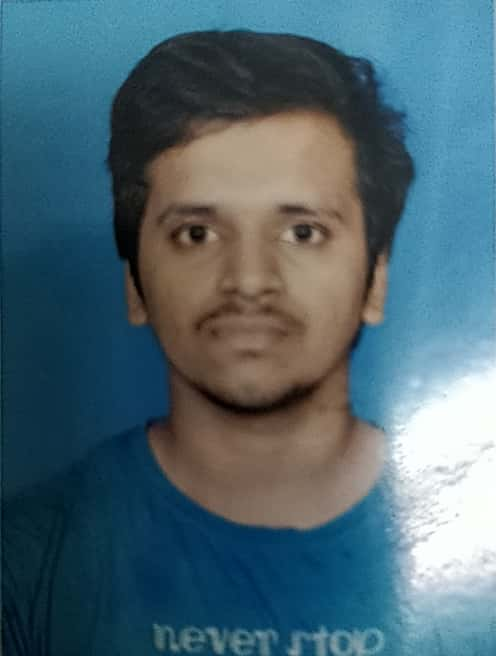
\includegraphics[width=2.5cm]{PHOTO1}
\end{wrapfigure} 
%------------------------------------------
\textbf{}  \\
\textbf{{\Large Smit Shah}}  \\
Email \hspace{0.2cm}  : smit08@somaiya.edu \\
Contact : 9757084146 \\
Address : 503,  5th Floor, Mauli Desire 1, Pushpa Park, Daftary Road \\
\hspace{1.8cm}Malad East, Mumbai - 400097 \\ 
%\textbf{}  \\
%------------------------------------------------------------------------------

%----------------------------Career Objective-------------------------------
\resheading{Career Objective}
\textbf{}  \\
A motivated Engineer with an aim to develop soultions for daily manual tasks through Automation and Roboitcs System \\

%-------------------Education--------------------------------------------------
\resheading{Education}

\begin{table}[h!]
  \begin{center}
      \begin{tabular}{l|c|r|l} % <-- Alignments: 1st column left, 2nd middle and 3rd right, with vertical lines in between
      \hspace{0.2cm}\textbf{Year}\hspace{0.2cm} &\hspace{0.2cm} \textbf{Degree/Certificate}\hspace{0.2cm} &\hspace{0.2cm} \textbf{Institute}\hspace{2.3cm} &\hspace{0.2cm} \textbf{CGPA / Percentage}\hspace{0.2cm}\\
      \hline
       2012 & \hspace{0.2cm} Secondary School Certificate \hspace{0.2cm} & \hspace{0.2cm}Children's Academy\hspace{1.7cm} & \hspace{1.2cm} 88.0\% \hspace{0.2cm}\\
       2014 & \hspace{0.2cm} Higher Secondary School Certificate \hspace{0.2cm} & \hspace{0.2cm}T.P.Bhatia College of Science\hspace{1.7cm} & \hspace{1.2cm} 76.72\% \hspace{0.2cm}\\
      2014 & \hspace{0.2cm} 1st Semester Btech ETRX \hspace{0.2cm} & \hspace{0.2cm}K.J. Somaiya College of Engineering\hspace{0.2cm} & \hspace{1.2cm} 5.96\hspace{0.2cm}\\
		2015 & \hspace{0.2cm} 2nd Semester Btech ETRX \hspace{0.2cm} & \hspace{0.2cm}K.J. Somaiya College of Engineering\hspace{0.2cm} & \hspace{1.2cm} 6.04 \hspace{0.2cm}\\
		2015 & \hspace{0.2cm} 3rd Semester Btech ETRX \hspace{0.2cm} & \hspace{0.2cm}K.J. Somaiya College of Engineering\hspace{0.2cm} & \hspace{1.2cm} 6.09 \hspace{0.2cm}\\
		2016 & \hspace{0.2cm} 4th Semester Btech ETRX \hspace{0.2cm} & \hspace{0.2cm}K.J. Somaiya College of Engineering\hspace{0.2cm} & \hspace{1.2cm} 6.0 \hspace{0.2cm}\\
		2016 & \hspace{0.2cm} 5th Semester Btech ETRX \hspace{0.2cm} & \hspace{0.2cm}K.J. Somaiya College of Engineering\hspace{0.2cm} & \hspace{1.2cm} 6.83 \hspace{0.2cm}\\
		2017 & \hspace{0.2cm} 6th Semester Btech ETRX \hspace{0.2cm} & \hspace{0.2cm}K.J. Somaiya College of Engineering\hspace{0.2cm} & \hspace{1.2cm} 6.48 \hspace{0.2cm}\\
		2017 & \hspace{0.2cm} 7th Semester Btech ETRX \hspace{0.2cm} & \hspace{0.2cm}K.J. Somaiya College of Engineering\hspace{0.2cm} & \hspace{1.2cm} 6.91 \hspace{0.2cm}\\
		      
          \end{tabular}
  \end{center}
\end{table}

ETRX - Electronics Engineering \\

%--------------------------Projects----------------------------------------------------------------
\resheading{Projects}
\textbf{}  \\
\textbf{Autonomous Water Rover With Underwater Inspection System} (July 2018- Present): \\
An Autonomous Water Rover With and Underrwater Inspection System Installed with Sensors and Camera for Monitoring of Water Bodies and Inspection of Underwater Infrastructures. \\
\textbf{}  \\
\textbf{Welding Automation} (December 2017 - January 2018): \\
A  system designed for automation of Seam Welding Process At Larsen and Toubro Heavy Engineering based on PLC and SCADA using Laser Distance Sensor to aid workers and relieve them of the constant heat and stress endured during the process.
\textbf{}  \\
\textbf{}  \\
\textbf{Unrolling Machine} (December 2017 - January 2018): \\
A modular system designed for the rolling and unrolling of steel plate liners used in Chemical Burners, the system can be assembled and dismantled in 20 minutes and uses 24V DC motor for electrical Safety.
\textbf{}  \\
\textbf{}  \\
\textbf{SONAR using AVR and Matlab} (March 2016): \\
An ultrasound sensor mounted on a servo was used to get obstacles in a 180 degree field of vision and the results were plotted using matlab.
\textbf{}  \\
\textbf{}  \\
\textbf{Wireless Mobile Charger} (2017)\\
\textbf{}  \\
\textbf{}  \\
\textbf{Robocon} (November 2016 - March 2017)\\
\textbf{}  \\
\textbf{Visitor Counter} (Jan 2015-July 2015): \\
A simple visitor counter designed using 8051 microcontroller.
\textbf{}  \\
%--------------------------------------Internship and Trainings---------------------------------
\resheading{Internships and Trainings}
\textbf{}  \\
\textbf{1. Trainee at Larson and Toubro  Heavy Engineering Department (Dec 2017-Jan 2018)} \\
A seam welding automation system and a rolling and unrolling machine were designed. 
\textbf{}  \\
\textbf{}  \\
\textbf{2. Trainee at Ericsson India Pvt Ltd.  (June 2018-July 2018)} \\
Undertook a Drive Test on field in Malad Sector for maintenance of Mobile Towers and solve Customer Complaints. 
\textbf{}  \\
%--------------------------------------Positions of Responsibilty---------------------------------
\resheading{Positions of Responsibilty}
\textbf{}  \\
\textbf{1. Senior Member Team KJSCE Robocon (May 19 2016- June 19 2017)} \\
\begin{itemize}
  \item Guided the junior members of the hardware team
  \item Organised and taught in a workshop on robotics by team KJSCE Robocon
  \item In-charge of all circuits on the robot.
\end{itemize}
\textbf{}  \\
\textbf{}  \\


%--------------------------------------Certifications---------------------------------
\resheading{Online Courses Completed}
\textbf{}  \\


\begin{enumerate}
  \item Machine Learning (Coursera -- Dec 2018)
  \item Web Development and Java Script (Microsoft -- Dec 2018)
\end{enumerate}

%--------------------------------------Technical Skills---------------------------------
\resheading{Technical Skills}
\textbf{}  \\


\begin{enumerate}
  \item Software Platforms Used:\\
  	\begin{itemize}
  \item Python programming on RPI (Intermediate)
  \item Arduino Programming (Intermediate)
  \item HTML, JavaScript, CSS (Basic)
  \item TesnorFLow (Basic)
  \item Visual Studio (Basic)
  \item Matlab (Intermediate)
  \item Verilog (Basic)
  \item Siemens SCADA and PLC programming
\end{itemize}
  	
  \item Hardware Platforms : 
  \begin{itemize}
  \item AVR and Arduino
  \item Raspberry PI 3b
  \item BeagloBone Black
  \item Siemens PLC S71200
\end{itemize}
\end{enumerate}

%--------------------------------------Soft Skills---------------------------------
\resheading{Soft Skills}
\textbf{}  \\

\begin{itemize}
  \item Self Motivated
  \item Ability to Work Under Pressure 
  \item Time Management
  \item Teamwork
  \item Problem Solving
 \end{itemize}

%--------------------------------------Extra Curricular Activities---------------------------------
\resheading{Extra-Curricular Activities}
\textbf{}  \\

\begin{itemize}
  \item Cricket
  \item Painting and Sketching 
  \item Volunteering in Education domain
  \item Trekking 
\end{itemize}
 
%--------------------------------------Co-Curricular Activities---------------------------------
\resheading{Co-Curricular Activities}
\textbf{}  \\

\begin{itemize}
   \item Won the "Best Hardware" award at the eYantra Ideas Competition 2019 
   \item Qualified for the semi-finals of ongoing DST and Texas Instruments hosted IICDC contest 2018
 \item Stood First at Prakalpa 2019
\end{itemize} 

%--------------------------------------Personal Details---------------------------------
\resheading{Personal Details}
\textbf{}  \\
Father's Name : Nilesh Shah\\
Mother's name : Trupti Shah\\
Date of Birth\hspace{0.28cm} : 8th March 1997\\
Nationality   \hspace{0.68cm}: Indian \\
Marital Status\hspace{0.25cm}: Single\\

%--------------------------------------References---------------------------------
\resheading{References}
\textbf{}  \\
\begin{enumerate}
	\item \textbf{Mr. Avinash A Prabhudesai} \\ Assistant Professor\\Mechanical Dept.\\avinashp@somaiya.edu\\
	\textbf{}  \\
Prof. Avinash Prabhudesai is the project guide of my final year project "Autonomous Water Rover". His work in KJSCE includes a university grant project on a regenerative brake and a consultancy project on performance improvement of a sugarcane harvester. He is Faculty Advisor for KJSCE Robocon and has an US Patent for "Radiator Grille" which was granted in January 2017.
	\item \textbf{Mrs. Arati Phadke} \\ Associate Professor\\Electronics Dept.\\aratiphadke@somaiya.edu\\
	\textbf{}  \\ Prof. Arati Phadke was my eYIC mentor and My Project Mentor. She was the Head of Department of Electronics Engineering from May 2008 to June 2011 and Dean (Student’s Affairs ) from May 2005 to April 2008.
\end{enumerate}

%--------------------------------------Declaration---------------------------------
\resheading{Declaration}
\textbf{}  \\
I, Smit Shah declare that all the details in this document are true and a valid proof of the same will be made available if required.\\

\textbf{}  \\


\end{document}

